\documentclass[]{article}
\usepackage[table,xcdraw]{xcolor}
\usepackage[left=3cm,right=3cm,top=1cm,bottom=2cm]{geometry}
\usepackage{amsmath}
\usepackage{graphicx}
\usepackage{subcaption}
\usepackage{multirow}
\usepackage{adjustbox}
\usepackage[table,xcdraw]{xcolor}
\usepackage{longtable}

% Title Page
\title{Industrial Plant Monitoring}
\author{TRAN Trung Duc}
\begin{document}
	\maketitle
	\newpage
	\tableofcontents
	\newpage
	\section{Introduction}
	
	\section{Summary} \textcolor{red}{a Modifier - add image- shorter}
	\paragraph{}In order to monitor a nuclear power plant, the electricity company will use a UAS equipped with a thermal camera. The UAS will be deployed to make flights around the plant which locates in a rural zone. The drone does not fly across the plant and keep the distance of 200m from the plant. There is not any airport near the inspected area. The drones is 30 kg with the maximun dimension of 2m is designed to fly automatically and  beyond visual line of pilot during the whole operation at 30m above the ground. 
	
	\paragraph{}During the flight, the pilot observes the status of the drone and the highway in real time via the GCS computer. The pilot needs to carry out only three simple actions: start the flight, end the flight (back to stand by mode), go home. The data exchanged between the GCS and the aircraft is transmitted via a wireless communication system.
	
	\paragraph {} The aircraft is equipped with a video camera with the characteristics as follows:
	\begin{itemize}
		\item Resolution: 1920 x 1080
		\item Min. Angle of view: 140 degree. 	
	\end{itemize}

	\paragraph {} The aircraft is equipped with a thermal camera with the resolution of 640 x 640 px
	
	\section{Operation description}
	
	\subsection{Organization overview} \textcolor{red}{a Modifier - add management for security}
    The highway company is the operator of the UAS operation. In the company, the UAS will be operated by a team of 2 people:
    \begin{itemize}
    	\item A pilot is in charge of observing and controlling the flight via the GCS computers. 
    	\item The second pilot is in charge of carrying out vehicle preparation before the flight, visual observation during takeoff and landing moment. During the flight, the she/he observes the nuclear power plant via the GCS computers.
	\end{itemize}
	\subsubsection{Safety and Cyber-security} \textcolor{red}{a Modifier}
	\paragraph {} The Safety Managment System have not been integrated into the the organization.
	\subsubsection {Design and Production} 
	\paragraph{} The highway company is not responsible for the design and/production of the UAS. The UAS is designed and producted by SOGILIS company and its partners.
	
	\subsubsection{Screw Training}
	\begin{itemize}
		\item The two crews are trained by the manufactures to operate the system in the normal, abnormal and emergency situation. 
		\item The two crews have training in general knowledge and competence adequate for the operation (UAS regulation, UAS airspace operating principles, Airmanship and aviation safety,Meteorology, Navigation/Charts, UA knowledge, operating procedures). 
	\end{itemize}
	
	\subsubsection{Maintenance} 
	\begin{itemize}
		\item The maintenance of the system is carried out by the manufacturer - SOGILIS.
		\item The maintenance instructions, maintenance schedules and maintenance procedures are defined and documented by the manufacturers.
		\item  The maintenance log system is used to record all maintenance activities conducted.  
		\item All maintenance staff have undergone a training program defined by the manufacturers. 
	\end{itemize}
	
	\subsubsection{Crew}
	\paragraph{} The UAS is operated by a team of 2 crews: pilot and support staff. The duties and responsibilities  of each crew are described as follows:
	\subparagraph{Pre-flight}
	\begin{itemize}
		\item In the pre-flight phrase, the pilot is in charge of starting the system and checking for any anomaly  of GCS, autopilot, communication, sensors values, batteries, aviation chart via GCS and verifying the weather condition. The checking is logged in a document 
		\item In the pre-flight phrase, the second pilot is in charge of visually checking for any damages, wears or tears; deploying the system in the takeoff area; verifying that the takeoff area is clear. The checking is logged in a document. 
	\end{itemize}

	\subparagraph{Flight}
	\begin{itemize}
		\item After checking for any anomalies via the GCS, the pilot starts the flight by sending taking-off command to UAV via GCS. The pilot observes the status of flight and the feedback video. In case of emergency situation, the pilot is in charge of deciding whether or not to continue the flight (by getting UAV back to the pre-determined site or letting the UAV drop).
		\item In the flight phrase, the second pilot is in charge of observing the nuclear power plant. In case of an emergency situation, the second pilot in charge of carrying out any necessary actions on the field to ensure the safety of the plant and revoke the equipment (e.g call the guardians).
	\end{itemize}
	\subparagraph{Post - flight}
	\begin{itemize}
	\item After the flight, the pilot turns off the UAV. The pilot is in charge of carrying out the post analyses of the data stored on the GCS.
	\item After the flight, the second pilot checks for any damage, wear or tear before taking the UAV back to store. The support staff is in charge of carrying out the post analyses of the data stored on the UAV.
	\item Both the pilot and the second pilot are in charge of completing the post analysis report and report any technical anomalies to the manufacturer. 
	\end{itemize}

	\subsubsection {UAS Configuration Management} \textcolor{red}{a Modifier}
	\paragraph{} Any changes to the hardware and the software(parameter configuration, flight plan modification, software update) are designed or created by the manufacturer.
	\paragraph{} Any changes to the UAS are carried out by the manufacturer. The instructions and equipment for this task are defined and documented by the manufacturer. 
	\paragraph{} The log system is used to record all changes conducted on UAS.
	
	\subsection{Operational procedure description} \textcolor{red}{a Modifier}
	\paragraph{}To observe the nuclear power plant, the owner company deploy a unmanned aircraft. The aircraft will fly around the plant. 
	
	\paragraph{} The drone of 30kg is designed to fly automatically and  beyond visual line of pilot during the whole operation at 30m above the ground. The flights is made inside a predefined geographic zone of100 large around the plant (geo-fencing). The distance between the flight zone and the plan is 200m. \textcolor{red}{a Modifier- add image}
	
	\paragraph{}During the flight, the pilots could observe the status of the drone and the plant via the GCS computers. The pilot could perform only three simple actions: start the flight, end the flight (back to stand by mode), go home. 
	
	\subsubsection{Standard operating procedures}
	\paragraph{Pre-flight procedures}
	\subparagraph{Operating site location} : The flight area (sky and land) is checked in order to ensure that a safety flight could be carried out:
	\begin{itemize}
		\item Other aircraft operations: Check to see if there are any other aircraft 
		operations within the immediate vicinity such as local aerodromes, sky 
		diving sites etc.
		\item Public Access: Is there any public access to the site and surrounding 
		areas? What is the likelihood of encountering a member of the public?
		\item Weather conditions: The weather will be checked on the day of the flight as well as whenthe pilot arrives on site. If at anytimethe pilot feelsthat the weather could jeopardisethe safety of the flight he has the right to cancel/abort the operation. 
		\item Pre-notification: it will be necessary to notify any nearby Aerodrome and aircraft operating sites or the local police of any operations that we are undertaking. If the	flight is being conducted in or near Aerodrome traffic then notification must be given beforethe event to ensurethat the flight won’t have an impact on the operations of said Aerodrome.
	\end{itemize} 
	
	\subparagraph{Preparation and correct assembly of UAV}: the UAVs are unpacked from the store and set up in accordance to the manufacturer's instructions.
	
	\subparagraph{Pre-flight checks on UAS and equipment} Once the UAV has been unpacked and assembled, the support staff will give the devicce one final check before the flight to confirm that there are no defects that were missed or that were caused during transit or conservation. Then the pilot starts the GCS and checks the value of displayed parameters, flight map for any anomalies. 
	These checks are defined in a checklist provided by manufacturer. 
	
	\paragraph{Flight procedures}
	
	\subparagraph{Take-off}
	\paragraph{} Once all the pre-flight checks have been completed, the pilot starts the flight by pushing the 'takeoff' button on GCS. Receiving the command of the pilot, the UAV automatically takes off and fly up to the altitude of 30m. 
	\paragraph{} During takeoff, the UAV is observed by both the pilot and the support staff.
	
	\subparagraph{In-flight}
	\paragraph{} After reaching up the 30m altitude, the UAV follows the predefined trajectory in order to capture the video of highway.
	\paragraph{} The pilot concentrates on monitoring the flight status (attitude, altitude, batteries, position) and monitoring the high-way.  
	\paragraph{} The support staff concentrate on visually monitoring the flight on the field.
	
	\subparagraph{Landing} 
	\paragraph{} Once the predefined trajectory is completed, the UAV goes back the landing site and hover over ground at 150m. Then it automatically lands on the ground. Once the landing is completed, the pilot pushes the 'dis-arm' button in order to turn off all the motors. Then the support staff turn off the power of the UAV.
	\paragraph{} During landing, the UAV is observed by both the pilot and the support staff.
	
	\paragraph{Post-flight}
	\paragraph{} Once a flight has been completed the time of flight must be logged. This will include the start and end times of the flight and the duration. Also any incidents must be noted and logged.
	\paragraph{} Then the UAV is inspected for signs of wear and tear or damage. If any is found it must be recorded.
    \paragraph{} All the flight data and video data stored on the UAV will be downloaded. 
    \paragraph{} All flight data (store on the GCS and the UAV) will be analyzed by the pilot and the support staff. Any incidents must be noted, logged and reported to the manufacturer.
    
    \subsubsection{Abnormal operation and emergency procedures}
	\subparagraph{Malfunctions}
	\paragraph{} If any malfunction (communication, sensor, battery, controller,etc) is detected on the UAV then steps must be taken to immediately land the device safely at one of the designated landing sites. If the malfunction make a controlled landing is unavailable, the pilot must shutdown all motors and let the UAV drop within flight zone. In order to protect the people on the ground and the aircraft, the aircraft is equiped with a parachute which could be automatically or manually deployed.    
	\paragraph{} A list of possible malfunction and necessary procedures are documented and provided by manufacturer.  
	\subparagraph{Lost of control}
	\paragraph{} In the case that the aircraft is totally lost of control and the auto fail-safe function is failed, the pilot could stop the operation manually by push the fail-safe button.
	\subparagraph{Change in Weather}
	\paragraph{} During the flight the weather must be monitored at all times. If the pilot feels that rain or snow is imminent then he will take steps to return the UAV to the designated landing zone
	\subparagraph{Fire}
	\paragraph{} In the event of smoke or fire coming from the UAV the pilot must immediately return to the landing zone to assess the cause and severity of the incident.In the case of damage or fire to the battery a fire blanket must be used to cover the UAV and control the fire
	\subparagraph{Designated Landing Area Compromised }
	\paragraph{}In the event that the designated landing area is compromised the pilot will land the UAV at the secondary site. If both sites are compromised the support staff will try to clear the obstruction to allow the pilot to safely land
\section{UAS description}

\begin{figure}[!ht]
	\centering
	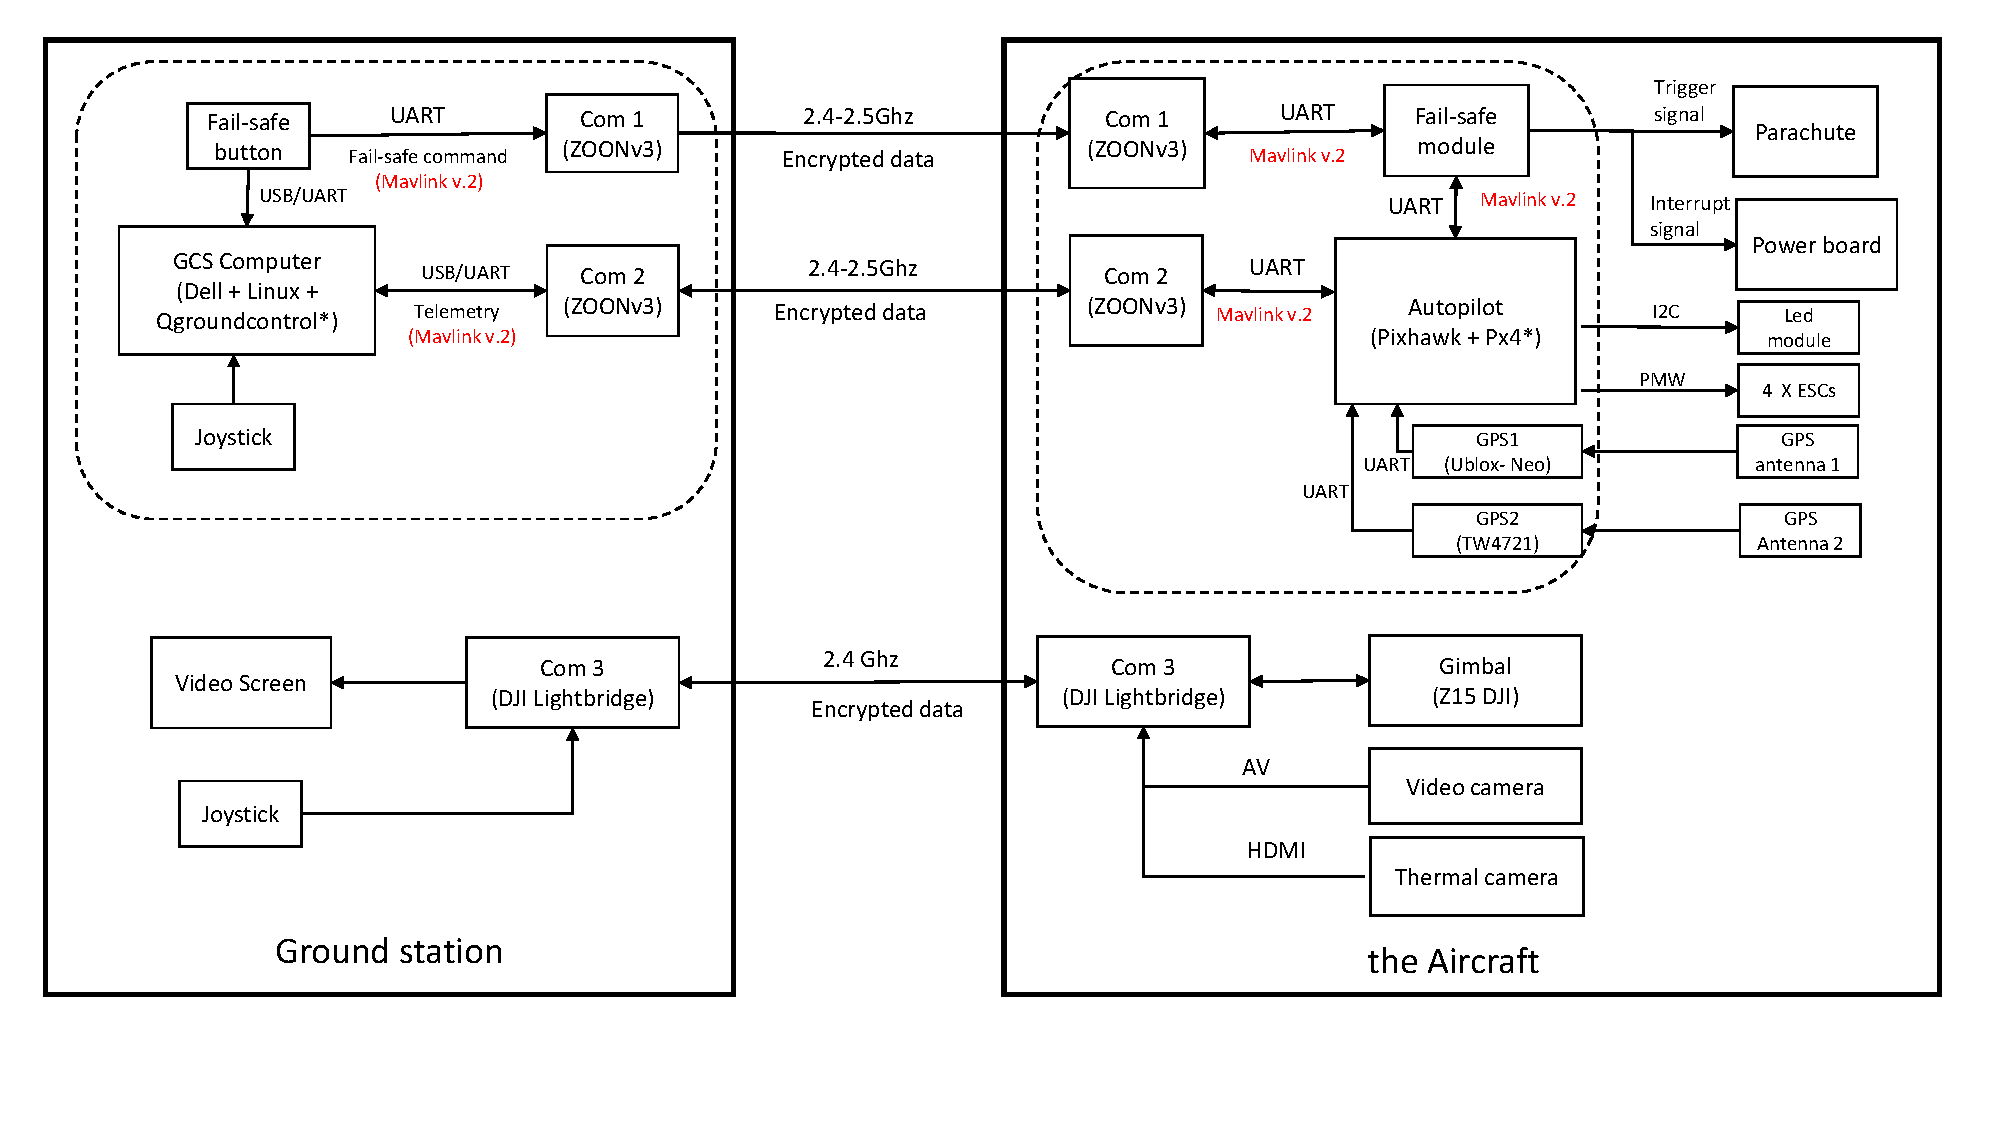
\includegraphics[width=0.9\linewidth]{drone_1.pdf}
	\caption{UAS Architecture}
\end{figure} 

\subsection{Ground Station}
\subsubsection{Ground control station computer}
The GCS computer is a DELL laptop installed the Linux operation and the Qgroundcontrol. The Linux operation provide a basic \textbf{access control} service. To access to the computer, the pilot has to have a account (identification + password). The Qgroundcontrol is a open-source GCS software. This software provide a user interface that allow the pilot to control and monitoring the status of the aircraft. The Qgroundcontrol is set up with the mavlink v2 communication protocol. GCS computer communicate with the aircraft via the Telemetry communication link - Com 2 (see \ref{sub:com}). The Qgroundcontrol software is modified to provide the supplemental cybersecurity functions presented in \ref{sub:cybersecurity}.
\subsubsection{Joystick 1}
The Joystick 1 provides pilot a measure to control manually the aircraft. The output of the joystick is sent to the aircraft via the GCS computer. The joystick connects to the GCS commputer via a USB port.
\subsubsection{Fail-safe button}
In the case that:
\begin{itemize}
	\item the aircraft fail to trigger automatically the fail-safe function 
	\item and the pilot could not also trigger manually this function via the joystick/ GCS computer    
\end{itemize}
The fail-safe button provide the pilot the final measure to trigger the fail-safe button. The output of the fail-safe button is sent to the aircraft via a emergency communication link - Com 1 (see \ref{sub:com})

\subsubsection{Module Com 1 \& Com 2 module}
See more detail in (see \ref{sub:com})
\subsubsection{Package}
The GCS commputer, joystick and fail-safe button and 2 communication module is packaged in a solid box to hide every unused connection ports.
\subsubsection {Video screen}
A screen is used to display the video recored by on-board camera.
\subsubsection{Joystick 2}
The joystick 2 provides the pilot a measure to control the cameras
\subsubsection{Com 3 module}
This module is a part of the communication link to stream the video from the aircraft to the ground. (see \ref{sub:com})
\subsection{Aircraft}
\subsubsection{Autopilot}
The autopilot includes the a pixhaw-based autopilot hardware and a Px4-based autopilot software. 
The autopilot hardware includes:
 \begin{itemize}
 	\item Main FMU Processor: STM32F765 32 Bit Arm® Cortex®-M7, 216MHz, 2MB memory, 512KB RAM
 	\item IO Processor: STM32F100 32 Bit Arm® Cortex®-M3, 24MHz, 8KB SRAM
 	\item On-board sensors:  2 x Accel/Gyro: ICM-20689 \& BMI055
 	\item Magnetometer: IST8310
 	\item Barometer: MS5611
 \end{itemize}

The autopilot software provides the aircraft the capacity of flying at auto mode and all required fail-safe functions.

In comparison with the original version, the autopilot is modified to provide the supplemental cybersecurity functions presented in \ref{sub:cybersecurity}.

\subsubsection{Fail-safe module}
The fail-safe module is used to trigger the parachute and the cut-off the motor power in case of emergency.

In the fail-safe case, the fail-safe module shall receive the command from
\begin{itemize}
	\item Autopilot
	\item or the fail-safe button on the ground via Com1
\end{itemize}

When receiving the fail-safe command, the fail-safe module shall send :
\begin{itemize}
	\item ``Trigger" signal to the parachute 
	\item ``Interrupt" signal to the power board (see \ref{subsub: power board}) to cut off motor power.
\end{itemize}

\subsubsection{GPS modules}
The aircraft is equipped with two different GPS modules : Ublox Neo and TW4721. This configuration create a redundancy for the safety of flight.

\subsubsection{ Com 1 \& Com 2 modules}
See more detail in (see \ref{sub:com})



\subsubsection {Package}
The Autopilot,  2 communication modules, the fail-safe module and 2 GPS modules is packaged in a solid metal box to hide every unused connection ports.

\subsubsection{Power board}
It distributes the electricity power from the battery to the motors and the electronic components.

In the fail-safe case, it shall cut-off the motor power.

\subsection{Communication} \label{sub:com}
\subsubsection{Com 1 \& Com 2}
The communication link 1 (Com 1) is used to send only the fail-safe command to the aircraft. The communication link 2 (Com 2) is for telemetry data. For these communication links, the ZOONv3 modules is used. The specification of these module is described as follows:
\begin{itemize}
	\item Range: 6km - 21km
	\item Frequencies:2.4-2.5Ghz
	\item Dataspeed: 0.5-256Kbps
	\item Encryption: ChaCha2.0
	\item Mavlink compatibility
	\item Tolerance to the decrease of the ommunication performance
\end{itemize}

\subsubsection{Com 3}
The communication link 3 is used for streaming video. The DJI Lightbridge is used for this link.

\subsection{Supplemental Cybersecurity features} \label{sub:cybersecurity}
\subsubsection{Autopilot software integrity}

For each time the parameters of autopilot or the source code of the autopilot are changed, the autopilot will create a encrypted hash of the source code and the parameters. This hash will be sent and stored in the GCS. 

When started, the autopilot generate a encrypted hash of the current source code and the current parameters. This hash shall be sent to GCS and compared with the hash stored in the GCS.  


\end{document}          
